\documentclass[../main.tex]{subfiles}

\begin{document}
	\subsection{Sprint 1}
	
	\par Der zweite Sprint wurde genutzt um das Grundgerüst des Spieles zu implementieren. Folgende User-Stories wurden vom PO definiert und vom Team bewertet:
	
	\begin{itemize}
		\item Hauptmenü erstellen
		\begin{itemize}
			\item Hauptmenüszene erstellen [2]
			\item Spiel starten [2]
			\item Spiel beenden [1]
			\item Spielszene erstellen [2]
			\item Zurück ins Hauptmenü aus der Spielszene implementieren [1]
		\end{itemize}
		\item Spielfeld erstellen
		\begin{itemize}
			\item Koordinatensystem bauen [5]
			\item Funktion für die Platzierung der Plättchen [5]
		\end{itemize}
		\item Plättchen-Stapel erstellen
		\begin{itemize}
			\item Plättchenstack implementieren [2]
			\item Nehmen des obersten Plättchen aus dem Stack implementieren [3]
		\end{itemize}
		\item Plättchen erstellen
		\begin{itemize}
			\item Plättchen-Objekt erstellen [2]
			\item Plättchentypen implementieren [2]
			\item Plättchenpunkte berechnen [5]
			\item Plättchen-Verhalten implementieren [3]
		\end{itemize}
		\item Review vom Sprint 0 schreiben [1]
		\item Evaluiere PVS Studio Static Analyzer für C\#/Unity [1]
	\end{itemize} 

	\par Die Tasks wurden alle bis zum Sprintende fertig gestellt.
	
	\begin{figure}[H]
		\centering
		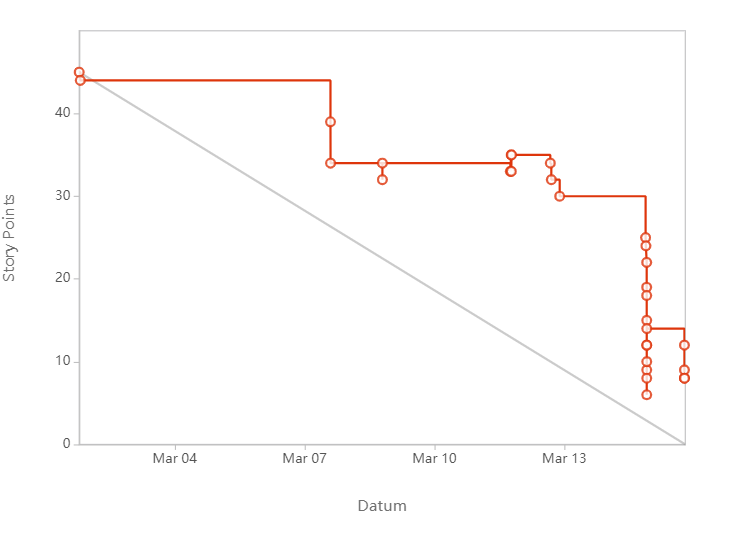
\includegraphics[width=0.5\textwidth]{Sprint_0_Burndown_Chart}
		\caption{Sprint 0 Burndown-Chart}
	\end{figure}

	\par Es gab initiale Schwierigkeiten, da ein Teammitglied am Anfang des Sprints das Team verliess. Er konnte aber seine Tasks noch vorzeitig beenden (einen grossen Dank dafür!) und verhinderte so jegliche Verzögerungen. Durch das eingehaltene Risikomanagement, wusste jedes Mitglied bereits im vornherein wie die implementierten Funktionen aufgebaut sind und konnte so die Velocity halten.
	
	\par Gleichzeitig wurde auch Entschieden, keine Ressourcen mehr in die Suche nach einem Static Analyzer zu investieren, da es zu viele ungenau definierte Optionen gibt und das Team diese Zeit lieber in die Entwicklung des MVP investiert.

\end{document}